\documentclass[a4paper,10pt]{article}
\usepackage[utf8]{inputenc}
\usepackage{ragged2e}
\usepackage{graphicx}
\usepackage{hyperref}
\usepackage{enumerate}
\graphicspath{/mnt/data_1/code/asignaturas/sint/practicas/pr7}
\newcommand\tab[1][1cm]{\hspace*{#1}}
\title{Sistemas Basados en Reglas\\(7ª semana)}
\begin{document}
\maketitle
\pagebreak
\tableofcontents
\pagebreak

\section{ejercicio 1}
\subsection{enunciado}
Sea el siguiente conjunto de reglas:\\
\vspace{0.5cm}\\
R1: Si h8 y h6 y h5 entonces h4 \\
R2: Si h6 y h3 entonces h9 \\
R3: Si h7 y h4 entonces h9 \\
R4: Si h8 entonces h1 \\
R5: Si h6 entonces h5 \\
R6: Si h9 y h1 entonces h2 \\
R7: Si h7 entonces h6 \\
R8: Si h1 y h7 entonces h9 \\
R9: Si h1 y h8 entonces h6 \\
\vspace{0.5cm}\\
La base de hechos inicial contiene h7 y h8. \\
\vspace{0.5cm}\\
Aplica encadenamiento hacia adelante suponiendo que se utiliza el principio de refracción y el control del razonamiento da mayor prioridad a la regla\\
a) con menor sub índice, y\\
b) con más condiciones en su antecedente (en caso de empate, tiene preferencia la regla de menor índice). Para cada iteraci ó n del sistema, indica las reglas que est á n activas y los hechos que la activan, la regla que se dispara y la base de hechos resultante.
\subsection{resolucion}
Sean las reglas que se satisfacen (inicialmente)
\vspace{0.5cm}\\
R4: Si h8 entonces h1 \\
R7: Si h7 entonces h6 \\
\vspace{0.5cm}\\
De estos sacamos la activación de 'h1' y 'h6'\\
Teneiendo activos los hechos h1 ,h6 ,h7 y h8
\vspace{0.5cm}\\
R5: Si h6 entonces h5 \\
R8: Si h1 y h7 entonces h9 \\
R9: Si h1 y h8 entonces h6 \\
\vspace{0.5cm}\\
Sacamos los hechos h5 y h9\\
obteniendo los hechos h1, h5, h6 ,h7, h8 y h9
\vspace{0.5cm}\\
R1: Si h8 y h6 y h5 entonces h4 \\
R6: Si h9 y h1 entonces h2 \\
\vspace{0.5cm}\\
activandose h4 y h2\\
quedando h1, h2, h4, h5, h6 ,h7, h8 y h9\\
\vspace{0.5cm}\\
Quedando en una situación estable, quedando activas todas las reglas menos R3.\\
Respecto a los hechos, se generan todos menos el h3.\\

\section{ejercicio 3}
\subsection{enunciado}
El siguiente SBR utiliza el axioma del mundo cerrado. Pero, ¿debiera utilizar dependencia reversible o irreversible entre las diferentes condiciones del antecedente?\\
SI hayCorriente Y sePulsaBotón ENTONCES ordenadorEncendido;
\subsection{resolución}
El proceso seria Reversible, ya que dependiendo de que el ordenador este encendido o apagado (antecedente) el pc se apagará o encenderá.

\section{ejercicio 6}
\subsection{enunciado}
Sean el siguiente conjunto de reglas que se ejecutan en un SBR con encadenamiento haciaadelante, axioma de mundo cerrado, principio de refracción, variables multivaluadas, y basede hechos inicial.\\
{H1: x3=20, H2: x2=5, H3: x1=0}\\
R1: SI x2 < 50 Y x2 > 0 Y x3 > 15 Y conocido(x1) \\
\tab ENTONCES afirmar(x1= 2*x2 + x1)\\
R2: SI x2 < 15 Y x1 = 0 ENTONCES afirmar(x1= 3*x2)\\
Indica los valores de la variable x1 en las dos siguientes iteraciones, cuando el control del razonamiento utilizado da prioridad a las reglas de menoríndice, o utiliza el principio deespecificidad, o utiliza el principio de actualidad.
\subsection{resolución}
\begin{tabular}{ c  c  c  c}
	iteracion & prioridad de menor indice & especificidad & Actualidad\\
	\hline
	1 & (H1)X1=10 & ? & ? \\
	2 & (H1)X1=20 & ? & ? \\
\end{tabular}\\
\pagebreak
\section{ejercicio 5}
\subsection{enunciado}
Resuelve el siguiente problema diseñando un Sistema Basado en Reglas que pueda darrespuesta a la pregunta Paradoja de la esfera:\\
Sea una esfera perfecta cuyo radio es diez veces mayor al del sol.\\
Sea una cinta que rodea a la esfera por su ecuador sin dejar oquedad en ninguno de sus tramos.\\
Supongamos que aumentamos la longitud de la cinta exactamente un metro, y que
la oquedad que se produce entre la cinta y la esfera se distribuye uniformemente por toda ella.\\
Se pregunta: ¿cuáles de los siguientes objetos pueden pasar, sin necesidad de tirar de la cinta de ninguno de sus tramos, por la oquedad entre la ella y la esfera?, ¿nada, un folio de papel, una mano, una pelota de béisbol?\\
\vspace{0.5cm}\\
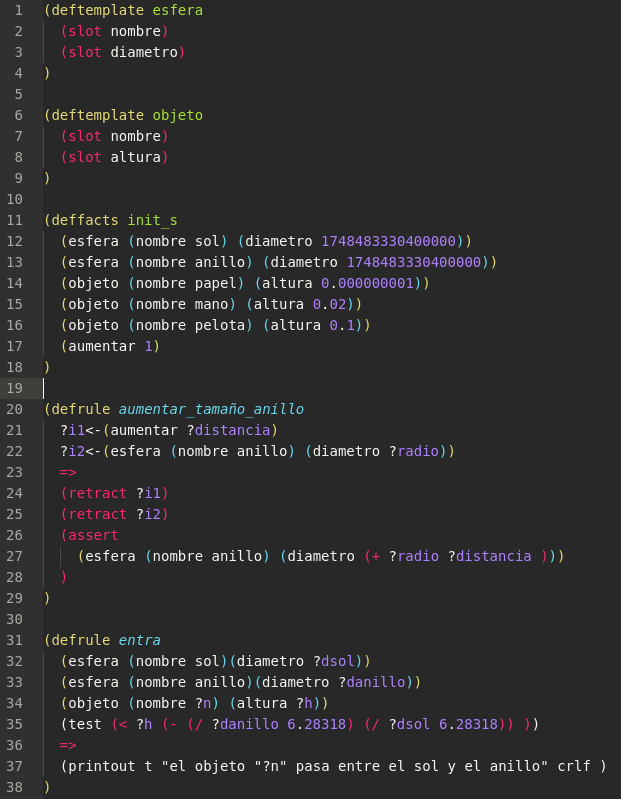
\includegraphics[scale=0.45]{code.png}




% \vspace*{\fill} %se va al final de  la pagina
% \raggedleft Documento escrito en \LaTeX{}
\end{document}
